\chapter{instalasi Docker di Server}

\section{Pembuka}

Panduan kali ini membahas cara instalasi docker di server. Server yang digunakan kali ini menggunakan sistem operasi 
Linux Ubuntu 21.04 dengan versi docker terbaru saat didokumentasikan yaitu 20.10.17. 

\section{Langkah Instalasi}

\begin{figure}
\subsubsection{1. Lakukan update paket pada linux} 
COMMAND : \textcolor{Blue}{sudo apt-get update}
        \begin{center}
          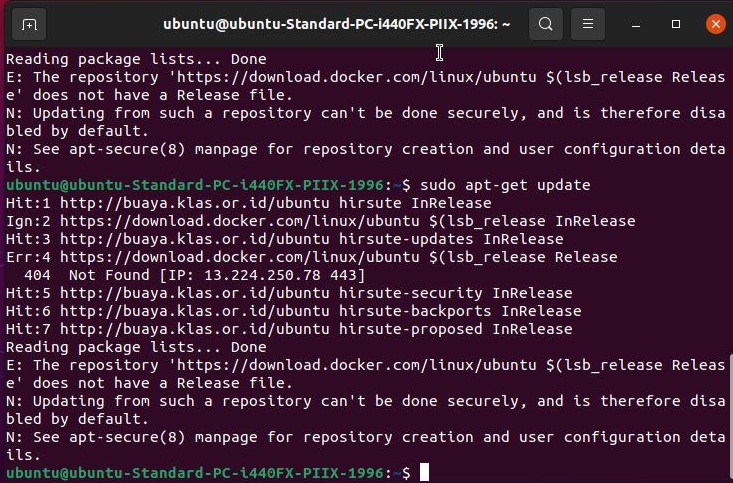
\includegraphics[width=\linewidth]{image/2.jpg}
          \caption{Apt update}
          \label{fig:my_figure}
        \end{center}
\subsubsection{2. Install paket yang memungkinkan apt menggunakan paket dari HTTPS}
COMMAND: \textcolor{Blue}{sudo apt install apt-transport-https ca-certificates curl software-properties-common}
        \begin{center}
          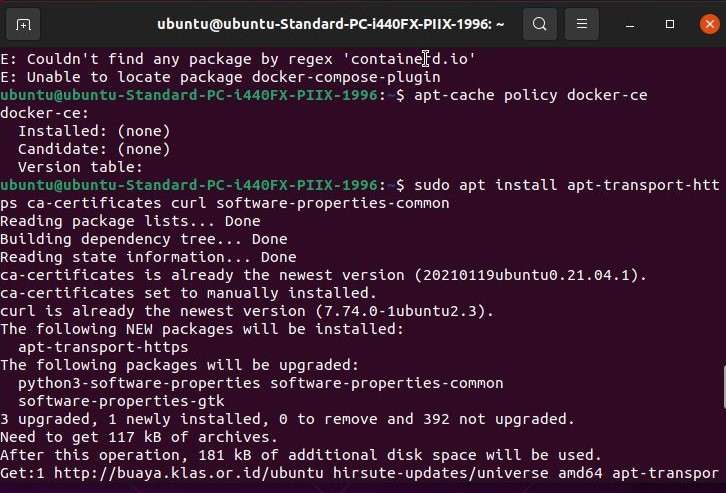
\includegraphics[width=\linewidth]{image/3.jpg}
          \caption{Apt menggunakan paket HTTPS}
          \label{fig:my_figure}
        \end{center}
\end{figure}

\begin{figure}
\subsubsection{3. Tambahkan kunci GPG untuk repositori resmi docker ke sistem dan lakukan update paket lagi}
COMMAND: \textcolor{Blue}{curl -fsSL https://download.docker.com/linux/ubuntu/gpg | sudo apt-key add –}

\textcolor{Blue}{sudo apt update}
        \begin{center}
          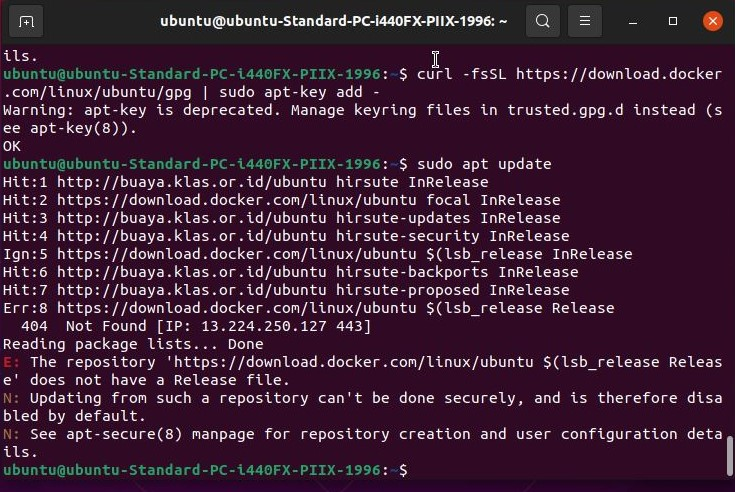
\includegraphics[width=\linewidth]{image/4.jpg}
          \caption{Tambahkan kunci GPG}
          \label{fig:my_figure}
        \end{center}
\subsubsection{4. Tambahkan repositori docker }
COMMAND: \textcolor{Blue}{sudo add-apt-repository “deb [arch=amd64] https://download.docker.com/linux/ubuntu focal stable”}
        \begin{center}
          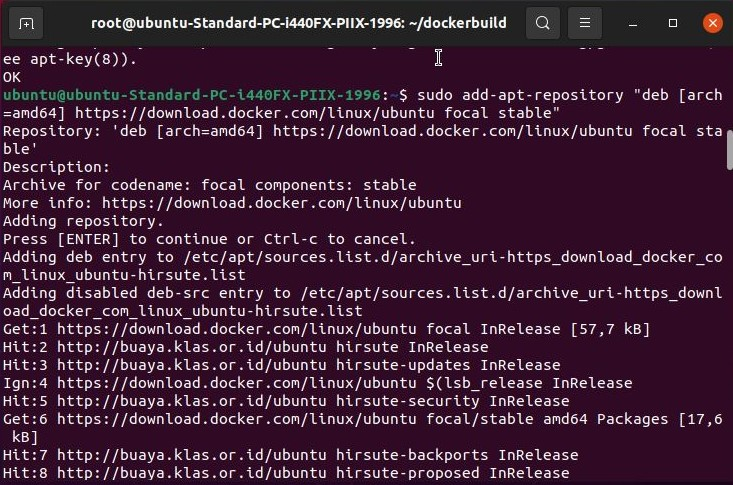
\includegraphics[width=\linewidth]{image/15.jpg}
          \caption{Tambahkan repositori docker}
          \label{fig:my_figure}
        \end{center}
\end{figure}

\begin{figure}
\subsubsection{5. Lakukan update paket lagi}
COMMAND: \textcolor{Blue}{sudo apt update}
        \begin{center}
          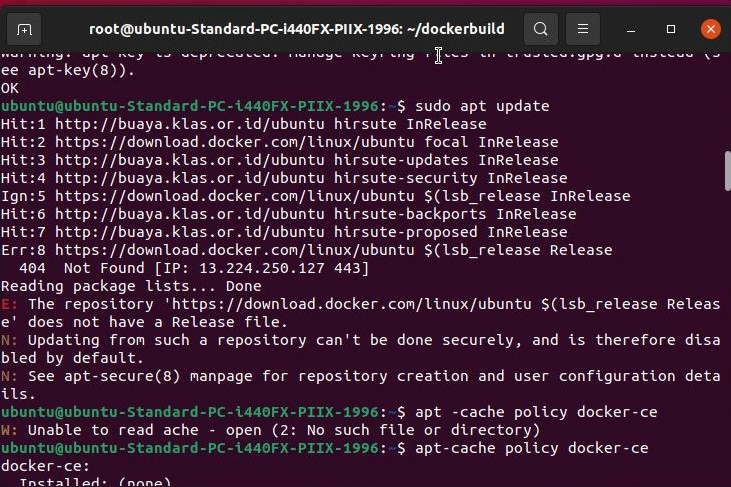
\includegraphics[width=\linewidth]{image/16.jpg}
          \caption{Update paket}
          \label{fig:my_figure}
        \end{center}
\subsubsection{6. Pastikan repositori instalasi docker dari repositori docker bukan ubuntu}
COMMAND: \textcolor{Blue}{apt -cache policy docker-ce}
        \begin{center}
          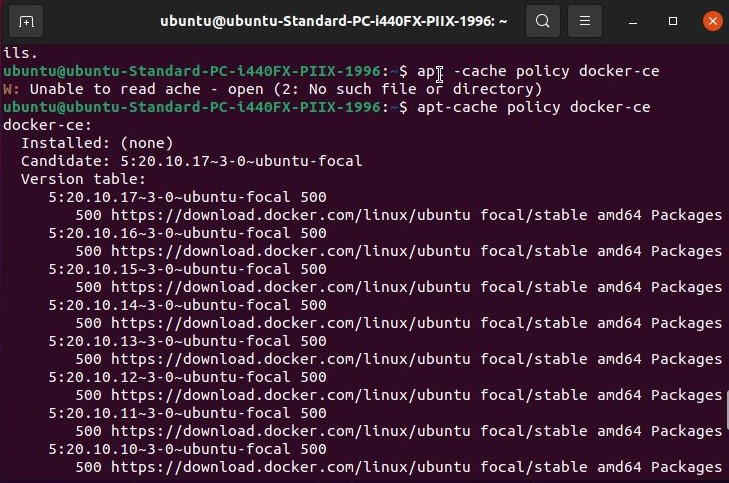
\includegraphics[width=\linewidth]{image/5.jpg}
          \caption{ Repositori instalasi docker dari repositori docker}
          \label{fig:my_figure}
        \end{center}
\end{figure}

\begin{figure}
\subsubsection{7. Lakukan instalasi docker}
COMMAND: \textcolor{Blue}{sudo apt install docker-ce}
        \begin{center}
          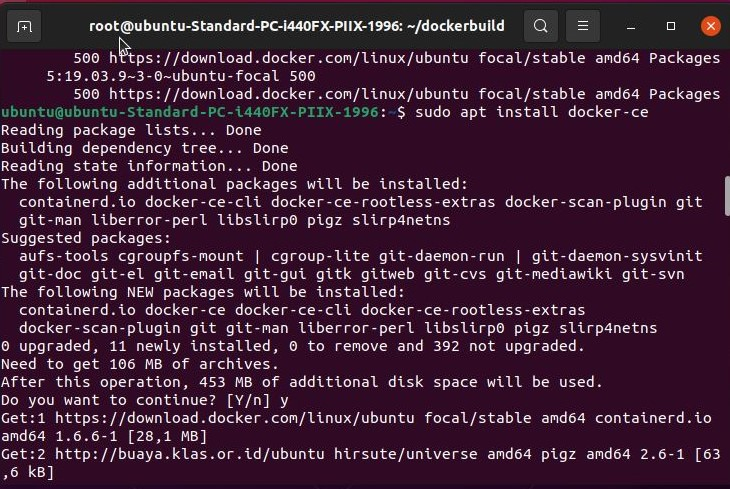
\includegraphics[width=\linewidth]{image/17.jpg}
          \caption{Instalasi docker}
          \label{fig:my_figure}
        \end{center}

\subsubsection{8. Pastikan docker berjalan}
COMMAND: \textcolor{Blue}{systemctl status docker}
        \begin{center}
          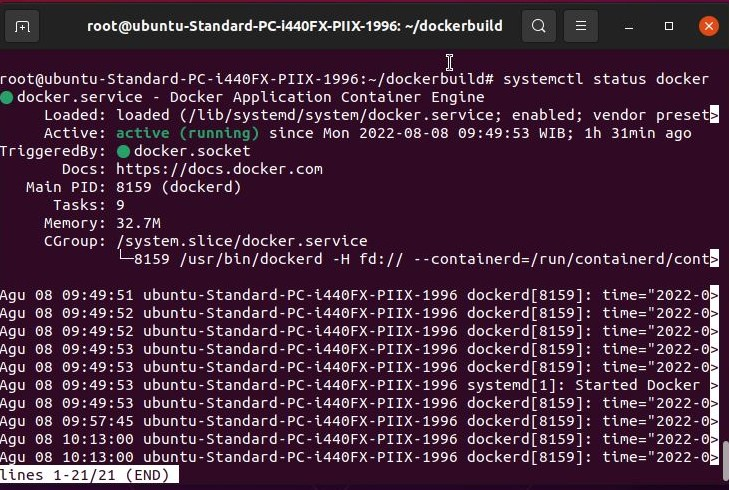
\includegraphics[width=\linewidth]{image/14.jpg}
          \caption{Memastikan docker berjalan}
          \label{fig:my_figure}
        \end{center}
\end{figure}